\begin{center}
Три причини да учите в Гимназия с преподаване на немски език „Гьоте":
\end{center}


\begin{itemize}
 \item Учебен процес осъществяван от висококвалифицирани преподаватели. Цялостната подготовка на учениците по немски език е ориентирана към Европейската рамка за чужди езици

 \item Развитие и усъвършенстване на уменията и компетентностите по всички предмети, което се доказва от отличните резултати от езикови изпити и ДЗИ

 \item Тясна връзка между преподаватели, ученици и родители

\end{itemize}

ГПНЕ „Гьоте" е едно от училищата в страната, партньори в инициативата PASCH, които с методическата и финансова подкрепа на Консултантския отдел по немски език от Федерална република Германия провеждат специализирано обучение по немски език. Учебните програми на МОН успешно се съчетават с рамковите изисквания за подготовката на изпита за придобиване на немска езикова диплома Sprachdiplom II (KMK).

Училищният учебен план осигурява задължителната и профилирана подготовка съгласно указанията на МОН, като отчита съвременните тенденции в образованието за връзка между изучаваните предмети и включва часове за работа по проекти. Вторият чужд език е английски. 

От 9 клас започва билингвално обучение - на немски и български език по биология и  химия. От 10 клас това обучение продължава по история и география.Наред с първи и втори профилиращи предмети - немски и английски език, в 11 клас се включва трети , а в 12 клас. 

Цялостната подготовка на учениците по немски език е ориентирана към Европейската рамка за чужди езици, като целта е в 12 клас да се достигне ниво С1 и да се положи успешно изпит за Немска езикова диплома Sprachdiplom. Гимназията е сред училищата в България, партньори по проекта "Училища, партньори на бъдещето."

Гимназията разполага с много добре оборудвани кабинети по всички учебни предмети, съобразени с модерната методика на преподаване и учене, мултимедийна зала, библиотека със специализиран отдел за DSD.  

Учителите на Немска гимназия, почти половината от тях бивши възпитаници на гимназията, са отлично подготвени преподаватели и поддържат европейското ниво на  образование. Признание за високите постижения на учители, административен и помощен персонал в гимназия "Гьоте" са много грамоти, сертификати, както и престижната награда "Димитър Бракалов". Резултатите на учениците в учебната дейност са впечатляващи - отлични постижения на Държавни зрелостни изпити, призови места в конкурси, състезания, олимпиади във всички културно-образователни области на общинско, регионално, национално и международно ниво, стипендии от Консултантски отдел при Посолството на Федерална република Германия, едногодишни стипендии за обучение в немски училища. Успехите се възнаграждават и претворяват в професионална реализация. 

Емблематичното изречение "Завършил съм Немската в Бургас" се е превърнало в гарант за качество. 4845 ученици вече са се доказали във всички сфери на обществения живот или са студенти в страната и чужбина. Години наред гимназията е център за провеждане на международни семинари за учители, преподаващи история, химия, биология, география на немски език, а от 1994 година- за първи път в Източна и Централна Европа тук се провеждат изпити за Немска езикова диплома, втора степен, на Конференцията на министрите на културата на Федерална република Германия. Година по-късно училището става изпитен център за Югоизточна България. 

Равносметката - 1646 ученици са завоювали немския сертификат, който им дава възможност да учат в немски университети, а шест ученици са спечелили стипендия за следване на Немската служба за академичен обмен.

Родителите са винаги съпричастни на училищните дела. Настоятелството е основано през 2001 година. То е достоен партньор във всички дейности на училището и подкрепа за Ученическия съвет, създаден през 2000 година. Възпитаниците на Немската гимназия продължават традициите на гимназията и с присъщия на младостта им устрем и замах осъществяват новите си идеи традиционният карнавал Фашинг, Мис и Мистър "Подготве", Коледни балове, Ден на тортата - всичко това - придружено от голяма доза смях, много вкус и умения. Но младите хора в гимназията са и социално ангажирани, с отворени сърца към хората с увреждания. С традиционните вече благотворителни концерти, Коледни и Великденски базари под надслов "Обич за всички" успяха да спечелят за доброто дело и връстниците си от другите езикови гимназии в Бургас. И са благодарни, не забравят, че самите те са получили подкрепа: компютри от Министерството на образованието, младежта и науката, Немски център, изграден и обогатен с Учителите на Немска гимназия, почти половината от тях бивши възпитаници на гимназията, са отлично подготвени преподаватели и поддържат европейското ниво на нашето образование. Признание за високите постижения на учители, административен и помощен персонал в гимназия "Гьоте" са много грамоти, сертификати, както и престижната награда "Димитър Бракалов". Резултатите на учениците в учебната дейност са впечатляващи - отлични постижения на Държавни зрелостни изпити, призови места в конкурси, състезания, олимпиади във всички културно-образователни области на общинско, регионално, национално и международно ниво, стипендии от Консултантски отдел при Посолството на Федерална република Германия, едногодишни стипендии за обучение в немски училища. Успехите се възнаграждават и претворяват в професионална реализация. Емблематичното изречение "Завършил съм Немската в Бургас" се е превърнало в гарант за качество. 4845 ученици вече са се доказали във всички сфери на обществения живот или са студенти в страната и чужбина. Години наред гимназията е център за провеждане на международни семинари за учители, преподаващи история, химия, биология, география на немски език, а от 1994 година- за първи път в Източна и Централна Европа тук се провеждат изпити за Немска езикова диплома, втора степен, на Конференцията на министрите на културата на Федерална република Германия. Година по-късно училището става изпитен център за Югоизточна България. Равносметката - над 1646 ученици са завоювали немския сертификат, който им дава възможност да учат в немски университети, а шест ученици са спечелили стипендия за следване на Немската служба за академичен обмен. Родителите са винаги съпричастни на училищните дела. Настоятелството е основано през 2001 година. То е достоен партньор във всички дейности на училището и подкрепа за Ученическия съвет, създаден през 2000 година. Възпитаниците на Немската гимназия продължават традициите на гимназията и с присъщия на младостта им устрем и замах осъществяват новите си идеи. 

Но младите хора в гимназията са и социално ангажирани, с отворени сърца към хората с увреждания. С традиционните вече благотворителни концерти, Коледни и Великденски базари под надслов "Обич за всички" успяха да спечелят за доброто дело и връстниците си от другите езикови гимназии в Бургас. И са благодарни, не забравят, че самите те са получили подкрепа: компютри от Министерството на образованието, младежта и науката, Немски център, изграден и обогатен с литература и материали със средства от гимназия "Гьоте", Дюселдорф, компютри, дарени от херцога на Бавария, Франц фон Байерн, съблекални и санитарни възли, реновирани със средства, дарени от гимназията в Молде, Норвегия, модерен кабинет по химия с финансовата подкрепа на Външното министерство на Германия и Община Бургас, дарения от бивши ученици на гимназията.

Подкрепата не се изразява само във финансови средства, а и в съвместни проекти с партньорите на немска гимназия от Румъния, Германия, Турция, Унгария: гимназия "Самуел фон Брукентал", Сибиу, гимназия "Агрикола", Кемниц, гимназия "Гьоте" Дюселдорф, гимназия "Хумболд", Гифхорн, , лицей "Шехид Осман паша", Ялова, гимназия "Аваши", Мишколц. Осъществените през годините проекти са зареждали учениците с много енергия и са били повод за изграждане на заслуженото им самочувствие, идващо от успехи в национален и европейски мащаб: европейски проект "Коменски" в Трабен-Трарбах, участие в Европейски конвент в Страсбург, проект на Франкфуртер Алгемайне Цайтунг "Младите хора пишат", проекти в Медиаш, Румъния, участие във фестивали в Булай, Германия, семинари по демократично образование, проект Eurocamp, проекти на Община Бургаслитература и материали със средства от гимназия "Гьоте", Дюселдорф, компютри, дарени от херцога на Бавария, Франц фон Байерн, съблекални и санитарни възли, реновирани със средства, дарени от гимназията в Молде, Норвегия, модерен кабинет по химия с финансовата подкрепа на Външното министерство на Германия и Община Бургас, дарения от бивши ученици на гимназията. Подкрепата не се изразява само във финансови средства, а и в съвместни проекти с партньорите на немска гимназия от Румъния, Германия, Турция, Унгария: гимназия "Самуел фон Брукентал", Сибиу, гимназия "Агрикола", Кемниц, гимназия "Гьоте" Дюселдорф, гимназия "Хумболд", Гифхорн, , лицей "Шехид Осман паша", Ялова, гимназия "Аваши", Мишколц. Осъществените през годините проекти са зареждали учениците с много енергия и са били повод за изграждане на заслуженото им самочувствие, идващо от успехи в национален и европейски мащаб: европейски проект "Коменски" в Трабен-Трарбах, участие в Европейски конвент в Страсбург, проект на Франкфуртер Алгемайне Цайтунг "Младите хора пишат", проекти в Медиаш, Румъния, участие във фестивали в Булай, Германия, семинари по демократично образование, проект Eurocamp, проект “Europe go green”,проекти на Община Бургас

\textbf{Ala Bala}

\begin{center}
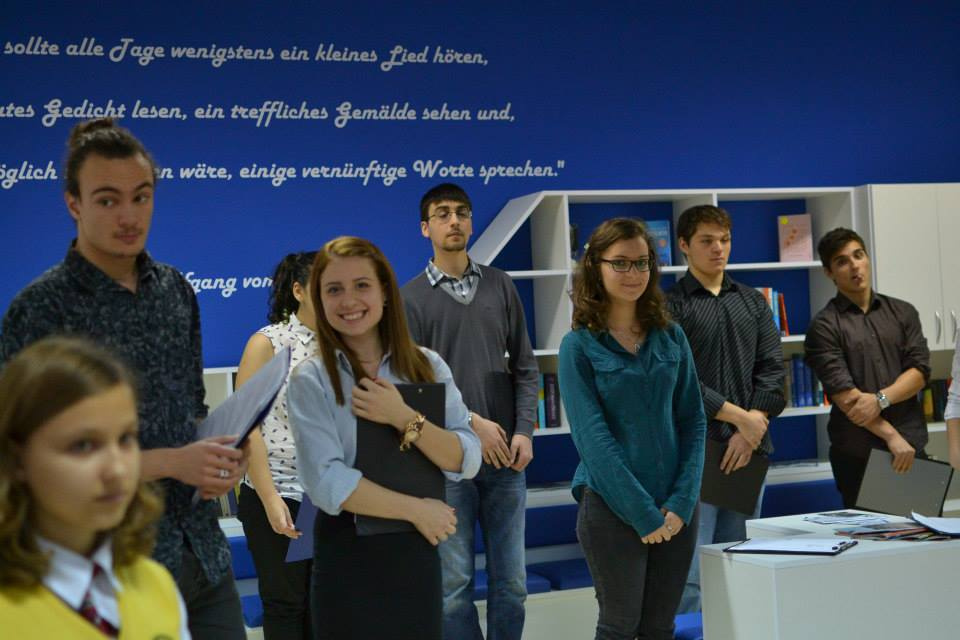
\includegraphics[width=6.0in]{./Reklama/fin.jpg}\\
\end{center}
\closearticle
